% Template for PLoS
% Version 3.4 January 2017
%
% % % % % % % % % % % % % % % % % % % % % %
%
% -- IMPORTANT NOTE
%
% This template contains comments intended 
% to minimize problems and delays during our production 
% process. Please follow the template instructions
% whenever possible.
%
% % % % % % % % % % % % % % % % % % % % % % % 
%
% Once your paper is accepted for publication, 
% PLEASE REMOVE ALL TRACKED CHANGES in this file 
% and leave only the final text of your manuscript. 
% PLOS recommends the use of latexdiff to track changes during review, as this will help to maintain a clean tex file.
% Visit https://www.ctan.org/pkg/latexdiff?lang=en for info or contact us at latex@plos.org.
%
%
% There are no restrictions on package use within the LaTeX files except that 
% no packages listed in the template may be deleted.
%
% Please do not include colors or graphics in the text.
%
% The manuscript LaTeX source should be contained within a single file (do not use \input, \externaldocument, or similar commands).
%
% % % % % % % % % % % % % % % % % % % % % % %
%
% -- FIGURES AND TABLES
%
% Please include tables/figure captions directly after the paragraph where they are first cited in the text.
%
% DO NOT INCLUDE GRAPHICS IN YOUR MANUSCRIPT
% - Figures should be uploaded separately from your manuscript file. 
% - Figures generated using LaTeX should be extracted and removed from the PDF before submission. 
% - Figures containing multiple panels/subfigures must be combined into one image file before submission.
% For figure citations, please use "Fig" instead of "Figure".
% See http://journals.plos.org/plosone/s/figures for PLOS figure guidelines.
%
% Tables should be cell-based and may not contain:
% - spacing/line breaks within cells to alter layout or alignment
% - do not nest tabular environments (no tabular environments within tabular environments)
% - no graphics or colored text (cell background color/shading OK)
% See http://journals.plos.org/plosone/s/tables for table guidelines.
%
% For tables that exceed the width of the text column, use the adjustwidth environment as illustrated in the example table in text below.
%
% % % % % % % % % % % % % % % % % % % % % % % %
%
% -- EQUATIONS, MATH SYMBOLS, SUBSCRIPTS, AND SUPERSCRIPTS
%
% IMPORTANT
% Below are a few tips to help format your equations and other special characters according to our specifications. For more tips to help reduce the possibility of formatting errors during conversion, please see our LaTeX guidelines at http://journals.plos.org/plosone/s/latex
%
% For inline equations, please be sure to include all portions of an equation in the math environment.  For example, x$^2$ is incorrect; this should be formatted as $x^2$ (or $\mathrm{x}^2$ if the romanized font is desired).
%
% Do not include text that is not math in the math environment. For example, CO2 should be written as CO\textsubscript{2} instead of CO$_2$.
%
% Please add line breaks to long display equations when possible in order to fit size of the column. 
%
% For inline equations, please do not include punctuation (commas, etc) within the math environment unless this is part of the equation.
%
% When adding superscript or subscripts outside of brackets/braces, please group using {}.  For example, change "[U(D,E,\gamma)]^2" to "{[U(D,E,\gamma)]}^2". 
%
% Do not use \cal for caligraphic font.  Instead, use \mathcal{}
%
% % % % % % % % % % % % % % % % % % % % % % % % 
%
% Please contact latex@plos.org with any questions.
%
% % % % % % % % % % % % % % % % % % % % % % % %

\documentclass[10pt,letterpaper]{article}
\usepackage[top=0.85in,left=2.75in,footskip=0.75in]{geometry}

% amsmath and amssymb packages, useful for mathematical formulas and symbols
\usepackage{amsmath,amssymb}

% Use adjustwidth environment to exceed column width (see example table in text)
\usepackage{changepage}

% Use Unicode characters when possible
\usepackage[utf8x]{inputenc}

% textcomp package and marvosym package for additional characters
\usepackage{textcomp,marvosym}

% cite package, to clean up citations in the main text. Do not remove.
\usepackage{cite}

% Use nameref to cite supporting information files (see Supporting Information section for more info)
\usepackage{nameref,hyperref}

% line numbers
\usepackage[right]{lineno}

% ligatures disabled
\usepackage{microtype}
\DisableLigatures[f]{encoding = *, family = * }

% color can be used to apply background shading to table cells only
\usepackage[table]{xcolor}

% array package and thick rules for tables
\usepackage{array}

% create "+" rule type for thick vertical lines
\newcolumntype{+}{!{\vrule width 2pt}}

% create \thickcline for thick horizontal lines of variable length
\newlength\savedwidth
\newcommand\thickcline[1]{%
  \noalign{\global\savedwidth\arrayrulewidth\global\arrayrulewidth 2pt}%
  \cline{#1}%
  \noalign{\vskip\arrayrulewidth}%
  \noalign{\global\arrayrulewidth\savedwidth}%
}

% \thickhline command for thick horizontal lines that span the table
\newcommand\thickhline{\noalign{\global\savedwidth\arrayrulewidth\global\arrayrulewidth 2pt}%
\hline
\noalign{\global\arrayrulewidth\savedwidth}}

\newtheorem{theorem}{Theorem}
\newtheorem{theorem2}{Theorem}
\newtheorem{theorem3}{Theorem}
\newtheorem{lemma}[theorem]{Lemma}
\newtheorem{axiom}[theorem]{Axiom}
\newtheorem{proposition}[theorem]{Proposition}
\newtheorem{corollary}[theorem2]{Corollary}
\newtheorem{definition2}[theorem3]{Definition}

% Remove comment for double spacing
%\usepackage{setspace} 
%\doublespacing

% Text layout
\raggedright
\setlength{\parindent}{0.5cm}
\textwidth 5.25in 
\textheight 8.75in

% Bold the 'Figure #' in the caption and separate it from the title/caption with a period
% Captions will be left justified
\usepackage[aboveskip=1pt,labelfont=bf,labelsep=period,justification=raggedright,singlelinecheck=off]{caption}
\renewcommand{\figurename}{Fig}

% Use the PLoS provided BiBTeX style
\bibliographystyle{plos2015}

% Remove brackets from numbering in List of References
\makeatletter
\renewcommand{\@biblabel}[1]{\quad#1.}
\makeatother

% Leave date blank
\date{}

% Header and Footer with logo
\usepackage{lastpage,fancyhdr,graphicx}
\usepackage{epstopdf}
\pagestyle{myheadings}
\pagestyle{fancy}
\fancyhf{}
\setlength{\headheight}{27.023pt}
\lhead{\includegraphics[width=2.0in]{PLOS-submission.eps}}
\rfoot{\thepage/\pageref{LastPage}}
\renewcommand{\footrule}{\hrule height 2pt \vspace{2mm}}
\fancyheadoffset[L]{2.25in}
\fancyfootoffset[L]{2.25in}
\lfoot{\sf PLOS}

%% Include all macros below

\newcommand{\lorem}{{\bf LOREM}}
\newcommand{\ipsum}{{\bf IPSUM}}

%% END MACROS SECTION


\begin{document}
\vspace*{0.2in}

% Title must be 250 characters or less.
\begin{flushleft}
{\Large
\textbf\newline{A simple model that explains why inequality is ubiquitous} % Please use "sentence case" for title and headings (capitalize only the first word in a title (or heading), the first word in a subtitle (or subheading), and any proper nouns).
}
\newline
% Insert author names, affiliations and corresponding author email (do not include titles, positions, or degrees).
\\
Renato Fabbri\textsuperscript{\Yinyang*},
Osvaldo N. Oliveira Jr.\textsuperscript{\ddag},
\\
\bigskip
São Carlos Institute of Physics, São Carlos, São Paulo, Brazil
\bigskip

% Insert additional author notes using the symbols described below. Insert symbol callouts after author names as necessary.
% 
% Remove or comment out the author notes below if they aren't used.
%
% Primary Equal Contribution Note
\Yinyang This author contributed with initial concepts, text, formalism and this final document.

% Additional Equal Contribution Note
% Also use this double-dagger symbol for special authorship notes, such as senior authorship.
\ddag This author contributed with formalism, senior authorship and this final document.

% Current address notes
% \textcurrency b Insert second current address 
% \textcurrency c Insert third current address

% Deceased author note

% Group/Consortium Author Note

% Use the asterisk to denote corresponding authorship and provide email address in note below.
* fabbri@usp.br

\end{flushleft}
% Please keep the abstract below 300 words
\section*{Abstract}
Inequality has always been a crucial issue for human kind,
particularly concerning the highly unequal distribution of wealth,
which is at the root of major problems facing humanity, including extreme poverty and wars.
A quantitative observation of inequality has become commonplace in recent years
with the expanding recognition that many natural and man-made systems can be represented as scale-free networks,
whose distribution of connectivity obeys a power law.
In this paper we introduce a simple model that explains the ubiquity of inequality,
based on two simple assumptions applied to a generic system with numerous parts.
In the first assumption we consider the components as being diverse, while the
second assumption is a uniform distribution of resources for the components.
This implies that the more resources are allocated per component, the less numerous are such components.
The second assumption is a conservation law: the amount of resources is conserved through component wealth.
This can be geometrically depicted as the distribution of object sizes in an n-dimensional Euclidean space.
Applying these assumptions to a generic system results in a power-law distribution,
whose exponent is the number of inputs that are independent from each other,
i.e. the dimensionality of the allocated resources.
Even though there is no restriction to the value of the exponent,
in practice we observe that existing systems normally exhibit an exponent between 1.5 and 3.0.
We indicate reasonable hypotheses for this limitation.
Since these assumptions are easily justified based on established knowledge,
the model proves unequivocally that inequality is ubiquitous.
We also discuss ways to control this tendency to inequality,
which is analogous to induce a decrease in entropy in a closed system by an external action.
% \section*{Author summary}
% Lorem ipsum dolor sit amet, consectetur adipiscing elit. Curabitur eget porta erat. Morbi consectetur est vel gravida pretium. Suspendisse ut dui eu ante cursus gravida non sed sem. Nullam sapien tellus, commodo id velit id, eleifend volutpat quam. Phasellus mauris velit, dapibus finibus elementum vel, pulvinar non tellus. Nunc pellentesque pretium diam, quis maximus dolor faucibus id. Nunc convallis sodales ante, ut ullamcorper est egestas vitae. Nam sit amet enim ultrices, ultrices elit pulvinar, volutpat risus.

\linenumbers

% Use "Eq" instead of "Equation" for equation citations.
\section*{Introduction}
Inequality has always been at the focus of social studies for the obvious importance for humanity and quality of life.
In some respects, inequality can be regarded as asymmetry, thus being at the center stage of science since symmetry is fundamental to cognition and knowledge in nearly all fields~\cite{deleuze,part}.
In fact, the ubiquity of symmetry is recurrent in the literature, according to which human thinking presents explicit, basic symmetry operations; therefore the world is modelled with symmetry regardless of its presence.
In recent years, inequality in distributions has been addressed quantitatively with more emphasis, particularly in large systems represented as networks.
Of special importance are the scale-free networks, whose distribution of connectivity (number of edges per node) obeys a power law
and whose
examples include human interactions, friendships, wealth, 
connections among airports and synaptic count between neurons~\cite{newman}.
Power laws also govern perception as expressed through the Stevens law
and other phenomena such as
earthquake intensity and allometric relations of animal bodies.
Incidence in basic physics is commonplace, e.g. in a Newtonian gravity force $F$ is related to distance $d$ through
$F=G\frac{m_1\;m_2}{d^2}$.
It is also known as the Pareto law and the most canonical example seems to be the Zipf law~\cite{newmanpower},
although the name ``Pareto law'' is often associated to power laws in the context of income or wealth~\cite{lada,economics}.
% Some advocate that data are better fitted with the superposition of a power-law distribution and a Weibull distribution~\cite{powWeib}.

We strove to keep this article as short and simple as possible, and the outline is as follows.
Next subsection is dedicated to relating previous work with the content here presented.
Section~\ref{sec:form} presents both an axiomatic and phenomenological description of the model.
Paradigmatic observations of the model are discussed in Section~\ref{sec:par},
while implications for wealth distributions are considered separately in Section~\ref{sec:esp}.
A case in which inequality is desirable is presented in Section~\ref{sec:meta}, which is followed by concluding remarks.

\subsubsection*{Related work}\label{sec:related}
Models with power laws for dealing with broad classes of phenomena have been extensively discussed~\cite{part,pbook,cereus},
but we could not find in the literature a truly unified framework for interpreting any power law, such as presented in this paper.
In fact, one may regard Self-Organized Criticality (SOC) as such a unified model, but SOC models presuppose that the system is a dynamical system~\cite{part}, as is the case for other models~\cite{slanina}.
Furthermore, most models are very specific to wealth (e.g.~\cite{bouchard}), meaning money and properties, while the simple model here presented is envisioned as way more general, and confluent with potentially any other model for power laws.
This is true for economic models in general and instances where power-law distributions are negated or restricted to special cases (in favor e.g. of the Boltzmann distribution) or to a portion of the population (e.g. 5-10\% richest)~\cite{arnab}.
Also, it is worth keeping in mind that not all models of wealth distribution result in power laws~\cite{dragulescu}, and that here the concept of wealth is wider than that of money and possessions. One may think of knowledge or health as a type of wealth in the following sections.

We argue that power laws, and their inherent extreme inequality, result potentially always from a uniform distribution of the resources, but even if they do not result from such uniform distribution, it is at least in agreement with it.
This is closely related to other models and even hinted by them, but not directly expressed as in the next section.
For example, many fractal-related models that result in power laws are akin to the example in Section~\ref{sec:siz}.

\section{Formalization}\label{sec:form}

\begin{definition2}
A complex system is a system in which the whole is more than the sum of the individual parts.
\end{definition2}

The definition of a {\bf complex system} and its components 
can otherwise be left open, given the broad range of definitions currently in use~\cite{complexity}.
For our purposes the system is generic and can have any type of component.

%Given the broad range of definitions currently in use, it seems
%more profitable to claim the commonsense notion of
%a complex system to be ``a system in which the whole is more
%than the sum of the individual parts'', and start with:

\begin{definition2}
	A {\bf resource} is anything that is used by a complex system to subsist and communicate.
\end{definition2}

In practice, a complex system is commonly delimited and specified through its components and the resources that it keeps. The resources are not restricted to any type and can be e.g. geometrical volumes, wave periods or currency values as illustrated in the following sections.

\begin{definition2}
	A {\bf resource-based system} is a complex system that has an underlying resource vital to their components and their interdependent roles.
\end{definition2}

%Specially in Game Theory, the components are often considered
%``self-interested''. This is not a required condition for the 
%framework here presented.
%Even so, we understand that this formalization shed insight
%in the reasons why and the ways that self-interested agents
%organize themselves
%with extensive incidence of power laws.

\begin{definition2}
	The {\bf component wealth} $k$ is the amount of resources (of any kind) allocated to a component.
\end{definition2}

We will use $p(k)$ to denote the fraction of components with component wealth $k$,
i.e. $p(k)$ will denote the probability of selecting at random a component with an amount $k$ of resources.
The correspondence among probability, frequency and relative count is
instrumental for the interpretative framework in this article,
which is conveniently embedded in the notation.
% It is also useful to regard $k$ as a wave period $\lambda$.
% Then, $p(k)$ is immediately understood as the frequency $f$.
% Note that $k$ is a measure of the resources, not total resources (or total component wealth), which might be correlated to $k$ and have $k$ as one of the resources.

\subsection{Propositions and corollaries}\label{propCol}
\setcounter{theorem}{-1}
\begin{proposition}\label{prop:0}
	There is diversity among the components of the resource-based system.
\end{proposition}

If there is a large set of components, there is hardly any way to avoid diversity. Be it location, size, age, the way someone regards them, etc., distinctions arise (as does symmetry). This can be regarded as a statistical law, or even as a deeper truth.
The mere existence of two objects imposes diversity, otherwise they would be both the same. Proposition~\ref{prop:0} is required for assigning different amounts of resources for each component: if they are equal, by definition they have the same wealth.

\begin{proposition}\label{prop:2}
	Resources allocation in a resource-based system is uniform across the incident component wealth. This is expressed as a uniform distribution $p_U(k)=C$ of resources with respect to component wealth $k$.
\end{proposition}

That is, resources are allocated democratically with respect to component wealth values, which has two major consequences: 1) the interval of incident component wealth is maximized with a constant resource $C$ distributed; 
2) the wealthier the components considered, the fewer they are. 
% Indeed, the resources are evidence for the persistence of the complex system under consideration, i.e. given a set of components the system is often delimited by the allocated resources and components without resources are discarded.

\begin{corollary}\label{prop:1}
	The different resource inputs are combined in the $\alpha$ dimensions of the resources.
%	The amount of each resource input to the system is fixed.
\end{corollary}
% If you observe one dimension k of an \alpha -dimensional resource,
% observe a C/k^\alpha distribution, regardless of which are
% the other dimensions: the \alpha-dimension relation
% of size and scale is preserved.

% If total resource = resource A x resource B ...
% they are all directly proportional to total resource


%Total resource is the product of resources in each dimension.
%
%Also, resources can be proportionally related.

This follows from the distinction of each resource dimension,
i.e. the incomparability of these amounts, say $\lambda_1$ and $\lambda_2$, and the multiplicative relation they hold with the total resource: $E=\widetilde{C_1} . \lambda_1 . \lambda_2 \equiv \widetilde{C_2}\lambda^{\alpha=2}$
with $\widetilde{C_X}$ constant.
Note that $E=\widetilde{C_1} . \lambda_1 + \widetilde{C_2}.\lambda_2 \equiv \widetilde{C_3}\lambda^{\alpha=1}$, that is: a resource resulting from the summation of other two unidimensional resources is a unidimensional resource. Therefore, one needs to use the product, not the sum. For example, if the resources are $workers$ and $time$,
a final resource $E=5\, workers + 4h=9$
holds little if any information, while
$E= 5\, workers \, . \, 4 h= 20\; workers . hours$ is
a reasonable measure of resources in a canonical metric.

\begin{corollary}\label{prop:3}
	The equilibrium state implied by the validity of Propositions~\ref{prop:0} and~\ref{prop:2} and Corollary~\ref{prop:1} is characterized by a power-law distribution $p(k)$ of components with component wealth $k$.
\end{corollary}

From the propositions, the same amount $C$ of resources is allocated
across all quantities $k$ of resources allocated per component.
Therefore, the fraction $p(k)$ of components with component wealth $k$ is
$p(k)=\frac{C}{k^\alpha}$, where $\alpha$ is
the dimensionality of the resources compared to the dimension of $k$.
As the system continues to exist,
and resources are continually allocated, deviations from the equitable distribution $p_U(k)$ of resources along component wealth $k$  tend to be transient. It is worth emphasizing that $p_U(k)$ is usually not made explicit in the literature, but only
 the power-law distribution $p(k)$ of components
with component wealth $k$.
%In other words,
%if there are $\alpha$ independent inputs,
%i.e. resources in $\alpha$ dimensions,
%each have a component wealth $k_n$ distribution
%$p_{k_n}(k_n)=C_n.k_n^{-1}$
%and the final and perceived distribution
%is the product of these functions
%%O = (R1*R2*… RN)/tN since a given input can be written as Ri/t. 
%$p(k) = \prod_1^{\alpha} C_n.k_n^{-1}\equiv C.k^{-\alpha}$. 

\begin{corollary}\label{cor:2}
  The extension of allocation is $[k_L,k_R]$ with $k_L$ often being 0 or 1 while $k_R\approx C^{1/\alpha}$.
\end{corollary}

This follows from Proposition~\ref{prop:2}.
If the allocation of resources is insensitive to component wealth,
it should sweep all possible values, and these usually
have a lower boundary by being a positive quantity of resources.
Systems are usually considered as a set of components
or the components in which certain resources couple them,
thus it is reasonable to assume $k_L=0$ or $k_L=1$.

The distributions $p(k)$ and $p_U(k)$ are also
bounded above when the component wealth reaches $k_R \approx C^{1/\alpha}$,
the amount of resources uniformly distributed along component wealth.
In empirical data, $k_R$ can vary considerably, due to
nonlinearity of the resources scaling (most often $k_R<C^{1/\alpha}$) and
to self-interested agents (most often $k_R>C^{1/\alpha}$).
Power laws are often reported to strictly conduct empirical data
only for a (broad) portion of component wealth range.

%\begin{corollary}
%	For a system with a finite quantity of resources,
%	the allocation is compact with a superior limit $k_2$.
%\end{corollary}

\begin{corollary}
  The upper limit $k_R$ of the observed allocation of resources is an estimate of the amount of resources $C$ equally distributed along component wealth ($C^{1/\alpha}\approx k_R$).
\end{corollary}

This follows from Corollary~\ref{cor:2}.

\begin{corollary}
	$N . p(1)$ provides another estimate of the amount of resources $C$ equally distributed along component wealth, where N is the number of components with $k=1$ ($C\approx N . p(1)$).
\end{corollary}

\begin{corollary}
	An estimate for $C$ can also be found by $\alpha$, $k_L$ and $k_R$ through Equation~\ref{eq:con} in the Appendix.
\end{corollary}

\begin{corollary}
	The dimensionality of the allocated resources is the scaling factor $\alpha$.
\end{corollary}

This last corollary follows from box counting or, most easily,
through wave-like reasoning about power laws, discussed in the next section.

\subsection{Phenomenological approach: power laws are consistent with the propositions}\label{sec:phen}
% pure mathematical interpretation of the power law

The propositions from the last subsection lead to power laws, and now we wish to verify whether phenomena governed by power laws are consistent with the propositions. In order to do that, we probe the definitions, propositions and corollaries from a more phenomenological standpoint, such as provided by empirical data. We take examples of 1D and 2D cases, and generalizations are straightforward.  


{\bf (1D case)} Consider a constant speed $v$ for a wave propagation with no dispersion.
Recall that the number of oscillations $f$ per unit time is
inversely proportional to the cycle length $\lambda$ (the period).
In usual notation $f=\frac{v}{\lambda}$.
The constant speed $v$ implies a power law between 
$f$ and $\lambda$ (with $\alpha=1$ and $C=v$).
This is the core insight: the general case of a power law can
be interpreted as resulting from a constant amount $C$ of
fundamental resources with dimensionality $\alpha$ 
being homogeneously distributed across
component wealth $k$ and resulting in $p(k)$ of such components.

{\bf (2D case and beyond)} Now let $f=\frac{v=C}{\lambda_1 . \lambda_2}$, that is, the frequency of occurrence
(or the probability of choosing such event at random) goes with the inverse of two periods while the speed is constant. 
If $\lambda_1==\lambda_2==\lambda$, then $f=\frac{v}{\lambda^2}$.
In other words, the density is given by an amount $v$
(or a quantity $C$ of resources) in a hypercube of
edge $\lambda$ (or component wealth $k$)
and $\alpha=2$ dimensions.
This reasoning yields the relative count, fraction or probability $p(k)$ of components with such component wealth $k$ and corresponding hypercubes $k^\alpha$.
Let $C_i$ be the amount of resources allocated at
specific resource costs,
and assume linearity $\lambda_{1,i}=c.\lambda_{2,i}$
such that
$p(k_i)=\frac{C}{C_i}=\frac{C}{\lambda_{1,i}.\lambda_{2,i}}=
\frac{C}{c\lambda_{2,i}^2}=\frac{\widetilde{C}}{\lambda_{2,i}^2}\equiv\frac{v}{\lambda^2}$.
Therefore, we only access $\lambda_1==\lambda_2$ and a ``normalized resource C'' allocated uniformly by the environment across component wealth: higher component wealth implies less numerous components. 

The cases above were related to phenomena represented by power laws.
For power-law distributions involving random variables, assume
random variables
$\lambda_{1,i}$ and $\lambda_{2,i}$ as possessing a uniform distribution of resources along component wealth
themselves:
$p_{\lambda_{1}}(\lambda_{1,i})=\frac{C_i}{\lambda_{1,i}^{\alpha_1}}$
and
$p_{\lambda_{2}}(\lambda_{2,i})=\frac{C_i}{\lambda_{2,i}^{\alpha_2}}$.
The product distribution of
$\lambda_{3,i}^2=\lambda_{1,i}.\lambda_{2,i}$
% is then:
% \begin{equation}\textstyle
% p_{\lambda_3^2}(\lambda_{3,i}^2)=C_1.C_2.\lambda_3^{-2\alpha_2}\frac{(R_{1,R}-R_{1,L})^{\alpha_2-\alpha_1+1}}{\alpha_2-\alpha_1+1}
% =C_1.C_2.\lambda_3^{-2\alpha_1}\frac{(R_{2,R}-R_{2,L})^{\alpha_1-\alpha_2+1}}{\alpha_1-\alpha_2+1}
% \end{equation}
is then:
\begin{align}
	p_{\lambda_3^2}(\lambda_{3,i}^2) = & \int_{-\infty}^{\infty} p_{\lambda_1}(\lambda_{1,i}) p_{\lambda_2}(\lambda_{3,i}^2/\lambda_{1,i})\frac{1}{|\lambda_{1,i}|}d\lambda_1 \\
	= & \int_{-\infty}^{\infty} p_{\lambda_2}(\lambda_{2,i}) p_{\lambda_1}(\lambda_{3,i}^2/\lambda_{2,i})\frac{1}{|\lambda_{2,i}|}d\lambda_2
\end{align}

\noindent whose integrals have non-trivial limits.
Note that $p_{\lambda_3^2}(\lambda_{3,i}^2)=\frac{N_i}{N}=p(\lambda_{x,i})$,
where $p(\lambda_{x,i})$ is the probability that a component has component wealth $\lambda_{x,i}$ and $N_i$ is the number of such components. 
% The number $N_i$ of components with component wealth $\lambda_{3,i}^2$ and the total
% number of components $N$ are conserved for $\lambda_{0,i}$.
% If one assumes $\lambda_{0,i} \propto \lambda_{3,i}$, then
% $p(k_{0,i}) \propto k_{0,i}^2$.


Together with the general model of Section~\ref{propCol}, this analysis amounts to a quasi-``if and only if'' mathematically grounded interpretation of any power-law relation.

\subsection{Introduction to an estimate of $\alpha$}
Consider a generic problem in which a System ($S$) provides an Output ($O$) depending on the Input ($I$) it receives.
Admit the following assumptions:
\begin{enumerate}
	\item $S$ is made of a number of components that are not all equal among themselves.
That is to say, there is diversity in the components, in accordance with Proposition~\ref{prop:0}. 
\item Distribution of resources is uniform with respect to the ``size'' of the components (component wealth) as in the geometric isotropic case of a house to be discussed in Section~\ref{sec:siz}.
This reflects Proposition~\ref{prop:2}
\item There may be several inputs, but for each input the amount of resources furnished to the System can be considered the same, 
	in accordance with Corollary~\ref{prop:1}.
\end{enumerate}

The Output ($O$)
is assumed to be the performance (or richness) in terms of the components of $S$.
If there are $\alpha$ types of independent inputs, i.e. resources in $\alpha$ dimensions,
the Output is the product of these inputs and should be
%O = (R1*R2*… RN)/tN since a given input can be written as Ri/t. 
$O =C.k^{-\alpha}$, where $k$ is a one-dimensional component wealth observation,
as shown in Section~\ref{sec:phen}. 

Let us illustrate with a hypothetical case.
Many tasks are to be done in a factory.
Assume three inputs:
number of workers $N$, working hours $W$
and efficiency $E$.
Sophisticated activities are developed by teams,
so we assume that all concentrations $C.k^3=n.w.e$
of these resources might be found in working groups.
Assuming the tasks change all the time,
all concentrations are important.
By Proposition~\ref{prop:2} they are equally important beforehand
in the sense that 
resources will be spread uniformly over $[k_L,k_R]$
with $p_U(k)=\frac{1}{k_R-k_L}$.
The number of such components, therefore,
decreases with $C.k^3=n.w.e$, the component wealth with three dimensions.
In other words,
$p(k)=\frac{C}{k^3}$, that is,
the fraction $p(k)$ of components (working groups) with component wealth $k$
decreases with $k^3$ and distributes the same
amount of resources $C=\frac{N.W.E}{k_R-k_L}$ along $k$.

The Output has therefore a power-law dependence on $k$ with exponent $\alpha$. Empirical values of $\alpha$
are normally between $1.5$ and $3$, from which one infers that there are fundamentally between two and three types of independent inputs to both natural and artificial systems. This can be envisioned, for a factory $S$, through resources of employees and time (the inputs I), with the fundamental resource being $person . hour$, the canonical resource for industrial production since the rise of Taylorism and taken to extreme limits in Fordism~\cite{fordism}.

\section{Paradigmatic observations of the propositions}\label{sec:par}
The interpretation of power laws presented in Section~\ref{sec:form} has an impact on the
understanding of
diverse systems.
Figure~\ref{tfig} is a fundamental representation of the model presented,
and should be kept in mind for reference while
selected phenomena are scrutinized in this section.

\begin{figure}[!h]
% 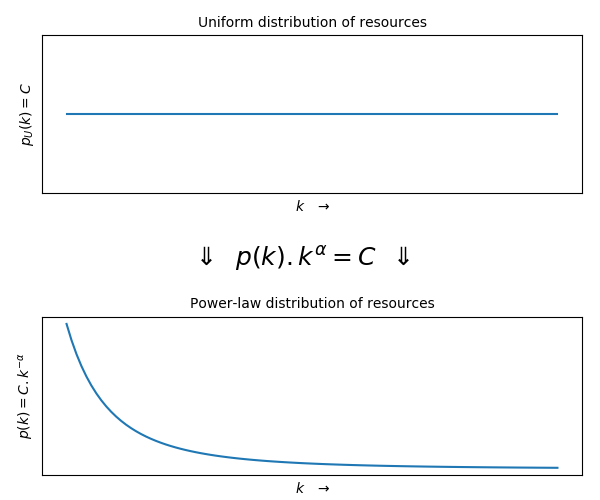
\includegraphics[width=3cm, height=4cm]{../scripts/uni2power}
  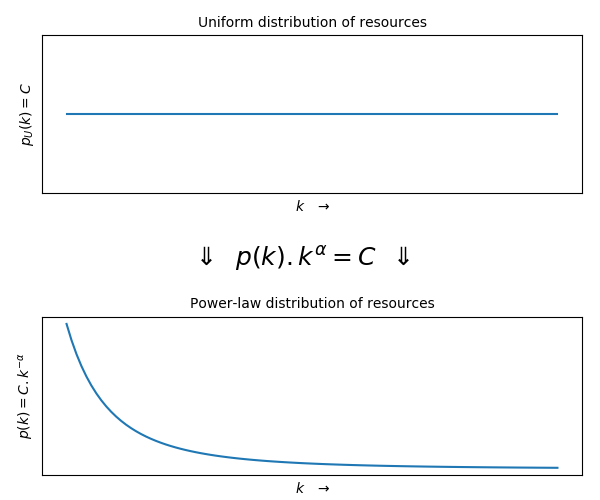
\includegraphics[width=0.7\textwidth]{../scripts/uni2power}
\caption{{\bf From uniform to power law.}
Let the system be insensitive to the amount of resources each component holds, i.e. let the amount of resources be conserved throughout the component wealth $k$.
  This assumption results in a power law if carried on in the terms described in Section~\ref{sec:form}.
  }
\label{tfig}
\end{figure}


 
\subsection{Object sizes in a house}\label{sec:siz}
Pick the size of a person (or the size of his/her hand, or  arm)
as a measure unit $l$ for length, pick $m \in (0,1)$.
In a house, there probably are more objects
of volume $\approx (m.l)^3$ 
than those of volume $\approx l^3$.
Furthermore, as we know nothing about the house,
we may assume that the chance $\rho$ of finding an object
within an arbitrary cube of volume $\approx (m.l)^3 \pm \beta(ml)$
is the same as finding an object fitting an
arbitrary cube of volume $\approx l^3 \pm \beta(l)$ for $\beta \in [0,1]$.
The house has a fixed volume so there are $m^{-3}$ more of
the smaller cubes and therefore $m^{-3}$ more objects of such
volume. 
The result is a power-law distribution of object volumes
related to the length $l$ with $\alpha=3$:
$p(l)=C.l^{-3}$.
If the objects are mutually exclusive,
$\alpha$ is probably lower, as the number of smaller
cubes decreases considerably.

This example holds a geometrical
interpretation of the formalism presented in the previous section.
It also might be assumed true even if there is no isotropy
and can be considered a ``best guess'' if total ignorance
about the system is assumed. 
Extreme choices of $l$ and $m$
might exhibit spurious observations
as the result of a bad fit of the scale for the analysis.

\subsection{Scale-free complex networks}

In a network, one has essentially $E$ edges and $N$ vertices.
Assuming linearity of resources:
\begin{equation}\label{eq:nre}
	Resources=C_1 N + C_2 E \approx C_2 E = C_2 N \frac{E}{N} = C_2 \frac{N \overline{k}}{2}
\end{equation}

\noindent where $C_1$ and $C_2$ are constants and $\overline{k}$ is
the average degree, i.e. the mean of the number of edges attached to each vertex.
If the nodes are not connected, they have minimized influence, also $N \ll E$ in most cases, thus the $C_1 N$ term is ignored.
Then:

\begin{equation}\label{eq:eqf}
	p_{E_i}(k_i)=\frac{C}{resources_i}=\frac{C}{C_2 E_i}=\frac{C/C_2}{N_i \frac{E_i}{N_i}}=\frac{2C/C_2}{N_i k_i} \equiv \frac{v}{\lambda_1   \lambda_2}
\end{equation}

% As $N_i$ and $k_i$ are both directly proportional to $E_i$, which is the fundamental resource,
This can be regarded as the case of social networks where the number of agents allocated $N_i$ and the time each of them put (related to $k_i$) are seen as the resource ($individuals . time$), and $\alpha\approx 2$
according to empirical evidence~\cite{newman}.

% Also:
% \begin{equation}\label{eq:eqf}
% 	p_{E_i}(k_i)=\frac{N_i}{N}=\frac{2C/C_2}{N_i k_i} \Rightarrow \frac{N_i^2}{N^2}=2\frac{C}{N.C_2}k_i^{-1} \Rightarrow p_{k_i}(k_i)\propto k_i^{-\frac{1}{2}}
% \end{equation}
% 
% \noindent so that if $p(k_i)$ is observed only with respect to the degree, 
% $\alpha=0.5$,
% which is far from empirical evidence because it only captures the distribution of one of the resources with respect to $k_i$.

\subsection{Natural laws}

Power laws are very recurrent in empirical data.
This already grants its place in the study of natural phenomena.
Different explanations are given for the many cases where
they are found, with most common denominators being fields such as
fractals, chaos, networks and unifying models e.g. as given by the Theory of Self-Organized Criticality~\cite{part}.
Cases in more traditional fields, such as Newtonian mechanics, where gravitational force relates to distance with $\alpha=2$ (if masses are fixed), are usually not mentioned in specialized literature about power laws, but regarded as very special phenomena e.g. related to mediation by massless particles.
In other words: there seems not to be a unifying theory of why power laws express such
an ubiquitous spectrum of relationships.

If the framework in Section~\ref{sec:form} is valid for all cases where power laws are found,
the consideration of power laws as tied to natural phenomena \emph{per se}, goes a step further. 
% Phenomenologically we have a fit (?) of the analysis.
That is: if there is
a power law, the analysis developed in Section~\ref{sec:phen} holds
and
the power law relation can be regarded as an equitable distribution
of resources in $\alpha$ dimensions.
If the acting of the ``laws'' given by Propositions~\ref{prop:0} and~\ref{prop:2} is fundamentally what is taking place, that should depend on phenomena
and standpoint.
We advocate that this framework deepens the understanding of potentially all power-law
incidences and is usually consonant with more explicit and intuitive 
relations of the system, its components and the context.
The core meaning seems to emanate, with the simplest formalism, from
the object sizes in the isotropic space described in Section~\ref{sec:siz}.
That is a reasonable geometric abstraction for
one to grasp the power-law inequality originated from
a uniform distribution
of fundamental resources through component wealth.
Also, relating power laws to the environment is the most effective
way we found to make explicit both the axiomatic
and the phenomenological backbones of the power-law ubiquity described in
Section~\ref{sec:form}.
We hypothesize that $\alpha \approx 2$ is due to two basic resources
input in any system: components and their time, energy or engagement.
All other resources seem correlated to these two.
We also hypothesize that deviations from $\alpha \approx 2$ are due
to other resources less correlated to them
or to any other nonlinearities in the relationship of resources.

\section{Implications for wealth distribution}\label{sec:esp}

One manifestation of inequality through power laws,
which is most fundamental to daily experience
in society, is found in the discrepant wealth distribution worldwide.
There are continuing efforts to deal with this issue,
usually advocating ways to minimize ``social inequality''.
Considering the framework presented within this article:

\begin{itemize}
	\item such inequality is a natural tendency that follows from Propositions~\ref{prop:0} and~\ref{prop:2} and is in accordance with the phenomenological discussion of Section~\ref{sec:phen}.
	\item Deviations from a power-law distribution of wealth should require work.
		Occasional deviations are part of the statistical aspect of the phenomena involved, but the maintenance of a pattern different from the power law derived from the resources distribution are fated to require the expenditure of energy.
	\item Both deviations of power laws towards a more equitable or towards a more unequitable distribution should be ephemeral or require work.
\end{itemize}

In particular, the (publicized)
homogeneity of earnings in public institutions,
and the (publicized) distribution of wealth in whole countries,
reveal that there is indeed efforts to minimize
the strong inequality imposed by power laws.
Additionally, publicized data should be regarded with
extra care and skepticism, as they do not always present the
expected power-law distributions.

In summary, power-law inequality seems to be an ubiquitous tendency
and a consequence of a distribution of wealth equitable and insensitive along wealth allocated to each component.
This implies the necessity of ``work'' for equalization.
Also, we observe that the higher the $k_L$ of equation~\ref{eq:pow}, the higher all the probabilistic mass will be located, which
implies greater wealth of the wealthier, the hubs or the ``elite''.
In other words, the richer the least rich,
the richer the more rich.
% It seems paradoxical that power laws, which are the current utmost inequality paradigm, follow from an equitable consideration of resource inputs as in Proposition 1.


\section{When inequality is desirable: the case of sensors and meta-sensors}\label{sec:meta}

Inequality is generally associated with negative implications, but unequal distributions may serve important, noble purposes, as in the example about perception we present here for the sake of the argument.  
Perception presents many psychophysical power-law relations between the magnitude of the physical stimulus and the perceived (subjective) quantity~\cite{pbook}. This can be attributed to the utility of perception, which is enhanced upon broadening of the spectrum of the perceived phenomenon. Another explanation is on the physical phenomena itself. Consider a sound wave traveling with constant speed $v$.
If the organism is susceptible to wavelengths from $\lambda_1$
to $\lambda_2$, $f=\frac{v}{\lambda} \in [\frac{v}{\lambda_2},\frac{v}{\lambda1}]$ follows a power law with $\alpha=1$. As made explicit in the discussion of Proposition~\ref{prop:2}, the power-law distribution
maximizes the component-wealth incident domain and,
therefore, the reception of signals.
In other words, the power-law inequality
maximizes versatility.

The existence of power laws in perception (and other sensing mechanisms) is advantageous, as acknowledged in the literature~\cite{psycho}. One may thus wonder whether complex systems with power-law behavior could be regarded as useful meta-sensors. By way of illustration, let us consider an interest group about hiking, which can be understood as a meta-sensor to find suitable 
places, equipment, people, proper behavior, etc.
The power law, i.e. ``the scale-free outline'' to use
the complex network jargon, sweeps a wide range of engagements (regarding the concentration of resources).
The higher the component wealth $k$, the higher the engagement,
but the lesser diversity is brought to the group
by the participant~\cite{tStable}: as one allocates more resources (say time) in one system, it allocates less resources in outside systems.

\section{Concluding Remarks}
The model presented here is based on simple propositions, and does not require the system components to be ``self-interested'',
unlike many other models leading to power laws (see a summary in~\cite{newmanpower,part}. Therefore, the formalization sheds light into in the reasons why and the ways that self-interested (and not self-interested) agents organize themselves with extensive incidence of power laws. The propositions in Section~\ref{propCol} can be thought of as laws met in a very broad class of phenomena and follow from the system complexity. Because there are so many mechanisms into play, we had to adopt assumptions that are very unlikely to be false. The resulting axioms can be understood as statistical tendencies that hold with such universality that they can be seen as laws that govern phenomena ubiquitously. 
Furthermore, the assumptions in the model lead to a framework analogous to the laws of thermodynamics:
conservation of resources and a time arrow pointing to inequality.

It is also worth emphasizing that physical laws expressed in the form of power laws and phenomena involving power-law distributions were treated on an equal footing. It remains to be seen whether such universality will be kept when specific problems are addressed. Still with regard to generality, if a complex system behaves according to the model proposed, then its energy will be related to the constant C of equation~\ref{eq:pow} for the distribution. Though we have not in any way treated the physical phenomena in complex systems in detail, one may speculate that if the Universe is composed of systems behaving as described in our model it might be possible to use the power-law concepts to seek for an explanation of dark matter or dark energy. 

Perhaps the most important implication of our findings is that inequality - implicit in power-law behavior - is a natural tendency for diverse natural and human phenomena. Of course, there are many deviations from power laws caused by nonlinearities. But in the overwhelming number of systems obeying power laws, deviations tend to be transient or require effort. We hypothesize that inequality may be minimizable by the expenditure of energy and that the characteristic $\alpha \in [2,3]$ is a consequence of the existence of two or three types of independent resources. Further work should link these findings to individual fields and contextualize the general framework.

\subsection*{Acknowledgments}
Financial support was obtained from the United Nations Development Program (UNDP, contract 2013/00056, project BRA/12/018);
the Brazilian National Counsel of Technological and Scientific Development (CNPq, process 140860/2013-4, project 870336/1997-5) and FAPESP (2013/14262-7).
The authors thank the Brazilian General Secretariat of the Republic Presidency (SG-PR) and all labMacambira.sf.net members for pursuing this and other developments.

\section*{Appendix: Power laws}
% \numberwithin{equation}{section}
\renewcommand\theequation{A\arabic{equation}}
\setcounter{equation}{0}
A power law is a functional relationship between two quantities $p(k)$ and $k$ in the form:
\begin{equation}\label{eq:pow}
p(k) = Ck^{-\alpha}
\end{equation}
\noindent where $k\in [k_L,k_R]$
and $C$ is constant.
There are four degrees of freedom in four characteristic variables:
$\alpha$, $C$, $k_L$ and $k_R$.
Suppose also $p(k)$ normalized so that
$\int_{k_L}^{k_R}p(k)=1$, i.e.
the power law is fit to represent a
probability density function.
Assuming idealized phenomena:
\begin{equation}\label{eq:con}
\int_{k_L}^{k_R}p(k)=1\;\Rightarrow\;
C=\frac{1-\alpha}{k_R^{1-\alpha}-k_L^{1-\alpha}}
\end{equation}

The cumulative distribution function $P(k)$, median $m$, mean $\mu$ and variance $\sigma^2$ are:

%\begin{equation}
%\begin{aligned}\label{eq:md}
\begin{align}\label{eq:md}
	P(k) &=\int_{k_L}^k p(\tilde{k})d\tilde{k}=\frac{C}{1-\alpha}(k^{1-\alpha}-k_L^{1-\alpha})=
	\frac{k^{1-\alpha}-k_L^{1-\alpha}}{k_R^{1-\alpha}-k_L^{1-\alpha}}\nonumber\\
	&\left ( m : \int_{k_L}^{m}p(k)dk=\int_{m}^{k_R}p(k)dk=\frac{1}{2} \right )\nonumber\\
	m&=\sqrt[1-\alpha]{k_L^{1-\alpha}+\frac{1-\alpha}{2C}}=
	\sqrt[1-\alpha]{k_R^{1-\alpha}-\frac{1-\alpha}{2C}}=
	\sqrt[1-\alpha]{\frac{k_R^{1-\alpha}-k_L^{1-\alpha}}{2}}\\
	\mu &= \int_{k_L}^{k_R}kp(k)dk=C\;\frac{k_R^{2-\alpha}-k_L^{2-\alpha}}{2-\alpha}=\left(\frac{1-\alpha}{2-\alpha}\right)\left(\frac{k_R^{2-\alpha}-k_L^{2-\alpha}}{k_R^{1-\alpha}-k_L^{1-\alpha}}\right)\nonumber\\
	\sigma^2 &= \left[ \int_{k_L}^{k_R}k^2p(k)dk=C\;\frac{k_R^{3-\alpha}-k_L^{3-\alpha}}{3-\alpha} =\left(\frac{1-\alpha}{3-\alpha}\right)\left(\frac{k_R^{3-\alpha}-k_L^{3-\alpha}}{k_R^{1-\alpha}-k_L^{1-\alpha}}\right) \right] -\mu^2\nonumber
%	m_n&=\frac{1}{N}\sum_{i=1}^N z_i^n \nonumber\\
%	R_n&=|m_n|\\
%	\theta_\mu&=Arg(m_1) \nonumber \\
%	\theta_\mu'&=\frac{T}{2\pi} \theta_\mu \nonumber
\end{align}
%\end{aligned}
%\end{equation}

Often, $k_R\rightarrow \infty$, $\therefore$

\begin{align}\label{eq:md}
	if \; k_R \rightarrow \infty \Rightarrow & & \nonumber\\
											      & if\; \alpha>1 \;\Rightarrow	& C = &\; \frac{\alpha-1}{k_L^{1-\alpha}}\nonumber\\
							   & & P(k) =& 1-\left(\frac{k_L}{k}\right)^{\alpha-1}\nonumber\\
										       &  & m  = & \sqrt[1-\alpha]{\frac{\alpha-1}{2C}}&=&\;\;k_L.\sqrt[\alpha-1]{2}&\\
							   & if\; \alpha>2 \;\Rightarrow	& \mu = & \;k_L^{2-\alpha}\frac{C}{\alpha-2}&= &\;\;k_L\frac{\alpha-1}{\alpha-2}& \nonumber\\
							& if\; \alpha>3 \;\Rightarrow	& \sigma^2 = & \;k_L^{3-\alpha}\frac{C}{\alpha-3}-\mu^2&= &\;\;k_L^2\frac{\alpha-1}{(\alpha-3)(\alpha-2)^2}&\nonumber
%	\mu = \int_{k_L}^{k_R}kp(k)dk=C\;\frac{k_R^{2-\alpha}-k_L^{2-\alpha}}{2-\alpha}\nonumber\\
%	\sigma^2  \int_{k_L}^{k_R}k^2p(k)dk -\mu^2 =C\;\frac{k_R^{3-\alpha}-k_L^{3-\alpha}}{3-\alpha}  -\left[C\;\frac{k_R^{2-\alpha}-k_L^{2-\alpha}}{2-\alpha}\right]^2\\
%	m : \int_{k_L}^{m}p(k)dk=\int_{m}^{k_R}p(k)dk=\frac{1}{2}
%	m_n&=\frac{1}{N}\sum_{i=1}^N z_i^n \nonumber\\
%	R_n&=|m_n|\\
%	\theta_\mu&=Arg(m_1) \nonumber \\
%	\theta_\mu'&=\frac{T}{2\pi} \theta_\mu \nonumber
\end{align}





\nolinenumbers

% Either type in your references using
% \begin{thebibliography}{}
% \bibitem{}
% Text
% \end{thebibliography}
%
% or
%
% Compile your BiBTeX database using our plos2015.bst
% style file and paste the contents of your .bbl file
% here. See http://journals.plos.org/plosone/s/latex for 
% step-by-step instructions.
% 
% \bibliography{../essay}

\begin{thebibliography}{10}
\bibitem{deleuze}
Deleuze G.
\newblock Difference and repetition.
\newblock Columbia University Press; 1994.

\bibitem{part}
Markovi{\'c} D, Gros C.
\newblock Power laws and self-organized criticality in theory and nature.
\newblock Physics Reports. 2014;536(2):41--74.

\bibitem{newman}
Clauset A, Shalizi CR, Newman ME.
\newblock Power-law distributions in empirical data.
\newblock SIAM review. 2009;51(4):661--703.

\bibitem{newmanpower}
Newman ME.
\newblock Power laws, Pareto distributions and Zipf's law.
\newblock Contemporary physics. 2005;46(5):323--351.

\bibitem{lada}
Adamic LA.
\newblock Zipf, power-laws, and pareto-a ranking tutorial.
\newblock Xerox Palo Alto Research Center, Palo Alto, CA, http://ginger hpl hp
  com/shl/papers/ranking/ranking html. 2000;.

\bibitem{economics}
Reed WJ.
\newblock The Pareto, Zipf and other power laws.
\newblock Economics Letters. 2001;74(1):15--19.

\bibitem{pbook}
Schroeder MR.
\newblock Fractals, chaos, power laws: Minutes from an infinite paradise.
\newblock Courier Corporation; 2012.

\bibitem{cereus}
Fabbri R, Pisani MM.
\newblock Egalitarian aspects of scale-free networks
\newblock Cereus UniRG; doi:10.18605/2175-7275/cereus.v10n4p98-106; 2018.

\bibitem{slanina}
Slanina F.
\newblock Inelastically scattering particles and wealth distribution in an open economy.
\newblock Physical Review E. 2004 Apr 14;69(4):046102.

\bibitem{bouchard}
Bouchaud JP, Mézard M.
\newblock Wealth condensation in a simple model of economy.
\newblock Physica A: Statistical Mechanics and its Applications. 2000 Jul 15;282(3-4):536-45.

\bibitem{arnab}
Sinha S, Chatterjee A, Chakraborti A, Chakrabarti BK.
\newblock Econophysics: an introduction.
\newblock John Wiley \& Sons; 2010 Nov 22.

\bibitem{dragulescu}
Dragulescu A, Yakovenko VM.
\newblock Statistical mechanics of money.
\newblock The European Physical Journal B-Condensed Matter and Complex Systems. 2000 Oct 1;17(4):723-9.

\bibitem{complexity}
Holland JH.
\newblock Complexity: A very short introduction.
\newblock OUP Oxford; 2014.

\bibitem{fordism}
Guill{\'e}n MF.
\newblock Models of management: Work, authority, and organization in a
  comparative perspective.
\newblock University of Chicago Press; 1994.

\bibitem{psycho}
Roederer JG.
\newblock The physics and psychophysics of music: an introduction.
\newblock Springer Science \& Business Media; 2008.

\bibitem{tStable}
Fabbri R, Fabbri R, Antunes DC, Pisani MM, de Oliveira Junior ON.
\newblock Temporal stability in human interaction networks.
\newblock Physica A: Statistical Mechanics and its Applications. 2017 Nov 15;486:92-105.

% 
% \bibitem{bib1}
% Conant GC, Wolfe KH.
% \newblock {{T}urning a hobby into a job: how duplicated genes find new
%   functions}.
% \newblock Nat Rev Genet. 2008 Dec;9(12):938--950.
% 
% \bibitem{bib2}
% Ohno S.
% \newblock Evolution by gene duplication.
% \newblock London: George Alien \& Unwin Ltd. Berlin, Heidelberg and New York:
%   Springer-Verlag.; 1970.
% 
% \bibitem{bib3}
% Magwire MM, Bayer F, Webster CL, Cao C, Jiggins FM.
% \newblock {{S}uccessive increases in the resistance of {D}rosophila to viral
%   infection through a transposon insertion followed by a {D}uplication}.
% \newblock PLoS Genet. 2011 Oct;7(10):e1002337.
% 
\end{thebibliography}



\end{document}

